\documentclass[a4paper,12pt]{article}

\usepackage[a4paper]{geometry}

\usepackage[utf8]{inputenc}            % Use utf8 input encoding
%\usepackage[latin1]{inputenc}         % Use iso 8859-1 encoding
\usepackage[T1]{fontenc}               % T1 fonts (support for accents/diacritics)
\usepackage{lmodern}                   % font with proper T1 support and good glyph quality

\usepackage{listings}                  % for (code) listings
\lstset{language=Java}
\usepackage{amsmath}                   % AMS math typesetting
\usepackage{titlesec}

\usepackage{hyperref}                  % better references for PDF

\usepackage{graphicx}               % for graphics
\usepackage{float}

\titleformat{\section}{\LARGE\bfseries}% hide redundant number
            {}{0pt}{}

\begin{document}

\begin{center}
	\rule{\textwidth}{0.1pt}\\[1cm]
	
	\Large Softwarepraktikum SS 2019\\\bf Assignment 1
\end{center}


\begin{center}

	\rule{\textwidth}{0.1pt}\\[0.5cm]

	{\Large Group - 6\\[5mm]}

	\begin{tabular}{lll}

		Roman Vuskov & 376809 & roman.vuskov@rwth-aachen.de \\

		Songran Shi & 357791 & songran.shi@rwth-aachen.de \\

		Marlene Damm & 379945 & marlene.damm@rwth-aachen.de \\
		
		Marvin Gazibarić & 378154 & marvin.gazibaric@rwth-aachen.de \\

	\end{tabular}\\[0.5cm]

	\rule{\textwidth}{0.1pt}\\[1cm]

\end{center}

% Uncomment next two lines for table of contents
%\newpage
%\tableofcontents

\section{Task 1}
Three playing fields have been created and uploaded to the $maps$ directory of the repository.

\subsection{compressedSquare.txt}

This is an $8$ player map utilizing transitions to create a $20\times20$ core, which fits in a $2\times2$ hole. This map could be achieved with less transitions but it will be interesting to see how the players handle the spacial disconnect. The mostly symmetrical design is supposed to ensure a fair game. Each player is presented with a multitude of possible moves from the get go.        

\begin{figure}[H]
    \centering
    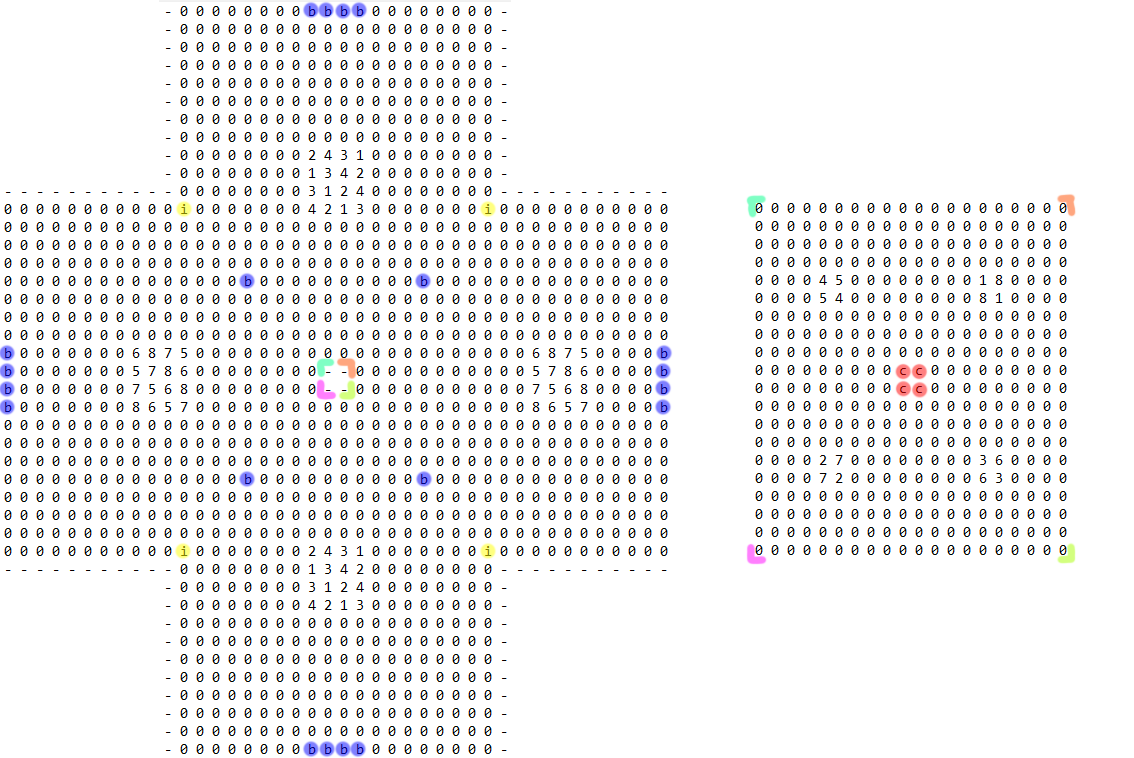
\includegraphics[height=11cm]{pictures/assignment1/compressedSquare.png}
    \caption{A representation of the playing field "compressedSquare" adjusted for transitions. The corners of the ASCII representation found in the repository are shown to actually be a connected square placed (through coloured transitions)  in the center of the cross shaped part.}
    \label{fig:compressedSquare}
\end{figure}



\subsection{starfish.txt}
This is an 8 player $33\times33$-map which has a lot of bonus fields which can be captured in the beginning phase of the game. So the players can gain an advantage respectively at the start. \\
There are transitions which connect the outer 17x4-fields with each other. These fields are isolated from the big field in the middle. This creates a separate playing field in which there are circles of neighbouring tiles. \\  
The outer corners of the map are connected, too. Thus there are nearly two circles with neighbouring tiles, which are separated only by the hole in the middle. For this reason it is possible to conquer a great amount of stone with one move.\\
One corner of each of the 4x4-fields it also connected to the hole in the middle of the big field. In this way there are more possible move for the player to conquer also the tiles which are part of the big field.
\begin{figure}[H]
    \centering
    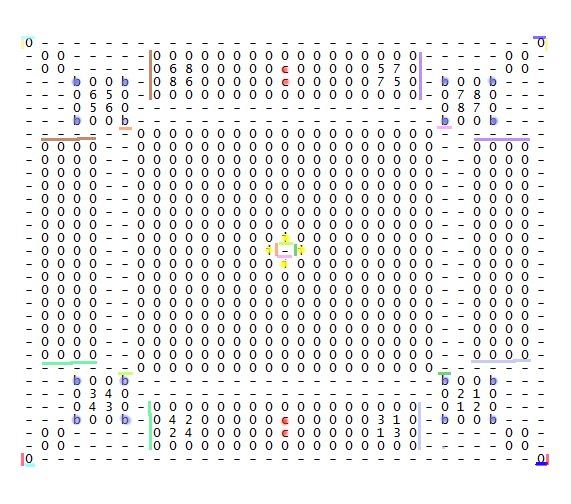
\includegraphics[height=11cm]{pictures/assignment1/starfish.PNG}
    \caption{A representation of the map starfish. The transitions and special fields are marked in colours.}
    \label{fig:starfish}
\end{figure}



\subsection{SierpinskiCarpet.txt}
An 8 player $27\times27$-map that visually resembles a Sierpinski carpet fractal, a mathematical object. The map is subdivided into 9 $9\times9$ medium squares, which in turn are subdivided into 9 $3\times3$ small squares. The center of each square has some special property that differs them from the rest of the square. The central medium square mostly consists of holes, interspersed with many bonus and choice tiles. The peripheral medium squares contain in their center either starting positions for players or easily accessible choice tiles. The rest of the map is scattered with access points to the central bonus tiles. These bonus tiles provide a powerful incentive for players to control the center of the map as soon as possible, leading to early interactions between players that are otherwise far apart. The access points in the periphery thus become strategically important locations in the process.



\begin{figure}[H]
    \centering
    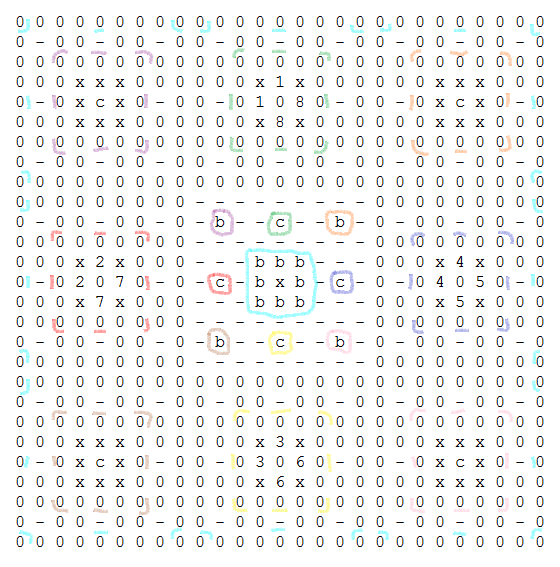
\includegraphics[height=11cm]{pictures/assignment1/SierpinskiCarpet.PNG}
    \caption{A representation of the map SierpinskiCarpet. The transitions and special fields are marked in colours.}
    \label{fig:SierpinskiCarpet}
\end{figure}

\section{Task 2}
The internal representation of the playing field is realized with the use by using several classes. Overall information like width, length and placement of tiles is stored in a \texttt{Map} object. Tiles are managed through a two-dimensional array. To extract one tile from this array \lstinline{getTileAt(int x, int y)} is used. A Map can be created using the static method \lstinline{readFromString(int width, int height, String[] lines)}. It reads a string array where each element contains a line of map data and creates a Map object with the according tiles from that.

Individual tiles are represented by instances of the \texttt{Tile} class. Each tile knows about its owner, its position on the map, whether it is a special field and which its neighbouring tiles are. This is necessary to store custom transitions and makes it easier to work with. Tile objects save their location on the map, enabling reverse-lookup in the two-dimensional array.

The realization of the tiles as a separate class makes it easier to gain access to the information which every tile contains and lets us easily expand the stored information, if that is required somehow in the future. Another possibility would be to write the information directly in separate two-dimensional arrays in the \texttt{Map} class, which then contain the information of the tile, but this is rather impractical to handle and on top of that it makes the code more confusing.

\section{Task 3}
Each move is represented by an object instance of a subclass of abstract class \texttt{Move}. There are two possible options to do a move in the first phase: either place an override stone or place a normal stone. 
The validation test routines of these two moves are similar. For this reason the abstract class \texttt{BuildMove} exists, containing the part that is shared between both move types. This class is extended by \texttt{RegularMove} and \texttt{OverrideMove}, both containing specific operations.

The validation test routine for the first phase first does a few checks to ensure that the given move is valid. It checks, whether the given tile is a hole, as no stones can be placed on holes.

To do an override move it is tested, if the destination tile is occupied. If not, the move is illegal. It is also tested, if the player has enough override stone left. If he has not, he is not allowed to override any stone. Moreover, an override move is not permitted to have any bonus request, because tiles which can be overridden, cannot have any special fields.

A regular move can only place stones on unoccupied tiles. It is also checked, whether the bonus request matches the property of the tile. For example it is not possible to request a bomb on a choice tile. The wrong combination of the tile property and the bonus request is declared illegal.

The test routine then does kind of a depth-first-search, following paths in every one of the eight directions. The direction of a path can change, if a transition points to another than the opposite direction on its destination tile. If there is a tile of the same number as the player's number on one of the paths, then the move is legal.\footnote{Given that the path does not end on the same tile it starts from.} The path ends when a tile is unoccupied or has no transition in the direction of search. If there is no path that leads to a tile of the active player, the move is illegal.

In the bombing phase, the  there is only one possible move, namely to throw a bomb. Those are represented by instances of \texttt{BombMove}.

The test routine for this second phase tests, if the player possesses a positive number of bombs. If not, the move is illegal. Also any bonus requests during the bombing phase are illegal. 

\section{Task 4}
The execution of the override move and the regular move are also very similar to each other. Therefore the superclass \texttt{BuildMove} implements the common parts of the algorithm for both moves, as in task 3.

The first step of the algorithm is to do a depth-first search in every one of the eight directions. As in task 3, the path for each direction is determined. If a path is a valid path that allows stones to be turned over, the path is traversed backwards and the stones are then actually turned over.

For an override move the algorithm decreases the amount of override stones the player has. If an expansion stone is overridden, the expansion property is removed from that tile.

For a regular move it is inevitable to also keep the special tiles in mind. If the tile is a bonus tile, the amount of bombs or override stones is increased by 1, depending on the attribute bonus request of the move.

A choice tile switches the tiles of the player with another player whose number is specified in the attribute bonus request. If that is the case, the algorithm traverses the map and searches for tiles having the number of either of both players, switching them each to the other one.

For the inversion tiles the algorithm traverses the map similarly and searches for tiles occupied by any player. The player reference of each tile, given as its number, is increased by one. The tiles belonging to the player with the highest player number are converted into tiles of player one.

After executing the effect of a choice or inversion tile, this special tile property is reset to default.

For a bomb move the algorithm determines the actually bombed tiles, being in the bomb radius. This is realized by breadth-first search. A list is used to save all affected tiles. The algorithm checks if a tile is already present in the list and does not add it twice.

At the end all tiles which are part of the List are bombed. Therefore the class Tile has a function which bombs itself. Tiles which are bombed turn to holes and their owner is reset. After that the transition from the neighbours to the bombed tile are removed and also the transition from the bombed tile to its neighbours. After the actual bombing process the number of bombs the player has, is decreased by one.

\section{Task 5}

The goal in this special version of the Reversi game is to achieve the highest rank, which means to be the player owning the most stones at the end of the game. If we had the computational power to construct the entire game tree from beginning to end, the evaluation of the leave nodes would consist of simply counting the amount stones we own. Like in many board games, however, this is not possible due to the exponential blowup of possible game states. In the following sections, we will analyze alternative heuristics that allow us to rate any board configuration.

An important property of our multiplayer game variant that applies to most of these heuristics should be noted here: Unlike the two-player variant where harming the opponent's position is equivalent to strengthening one's own position, here the weakening of a particular opponent's position is a public good to all the other opponents. A selfish agent therefore should \emph{not} seek to e.g.\ constrain an opponent's mobility at its own cost. The only exception to this is towards the end of the game when the rank of players is no longer expected to vary wildly, and one has only to worry about its closest competitors (those directly above and below the player's rank).

\subsection{Building Phase}

\subsubsection{Inverse and Choice Tiles}
Before we can move on to discuss specific heuristics, we must consider the inverse and choice tiles first - these game mechanics alter the game in such fundamental ways as to make other evaluation functions completely useless until they have been removed. As long as there are still inversion and/or choice fields left on the map, there will be great uncertainty about the very ownership of the stones. In fact, although this stage is technically part of the build phase, strategy-wise it is better to think of it as its own phase - let's call it the "Uncertainty Phase".

Consider, for instance, a map with 8 players and 2 inversion tiles where we are player 1. It appears very likely that all 4 inversion tiles will be captured at some point during the game since it seems rather impossible to defend them from all other players (especially with override stones in the game), and there isn't a strong incentive to do so anyway. One might suggest, then, that we ought to play moves that "benefit" player 7 the most since that's who's stones we'll be taking over eventually, but this is a rather futile effort since we have little influence on player 7's position. Who himself is trying to  player 5's position instead of his own according to the normal heuristics, of course.

A similar situation ensues in the case of choice fields: It is futile to optimize other evaluation functions since that would only make one more susceptible to player swaps. It's even pointless to go for choice fields ourselves but the last one since we'll still be vulnerable to swaps afterwards, and there most likely won't be worthwhile targets as no one is incentivized to play well and take the lead.

It seems the only objective in this uncertainty phase of the game is to capture as many bonus tiles as possible since they're not subject to swaps.


\subsubsection{Counting Stones}
A naive heuristic one might consider initially is to simply count the number of one's stones - after all, this is the decisive attribute at the end of the game. However, due to the possibility of overturning a large number of opponent stones in any given move, this value won't be very informative for almost the entire game. On the contrary - owning a large amount of stones early in the game might provide opponents with plenty of opportunity to place their stones right next to ours, boosting their mobility. This heuristic should therefore be discarded.

 
\subsubsection{Mobility}
We define mobility $m$ as the number of immediate legal moves available to the player in turn. As with most board games, keeping one's options open and not forced into Zugzwang is essential. 

 
\subsubsection{Stability}
According to the rules of Reversi, a stone can only be overturned (in regular moves) if an opponent catches it between two of his own stones on a straight line. There are only 4 directions for straight lines on a Reversi map: horizontal, vertical and the two diagonals. If a tile borders a hole in one of these 4 directions, any stone placed on this tile will be immune to capture in that direction - we say the stone has a stability of 1. According to this measure, stones on edge tiles have a stability of (at least) 3, and on corner tiles of the map even 4 - they're completely stable. Furthermore, bordering a stable stone of the same color will also make a stone stable in that direction. Lastly, if a straight line is completely filled with stones from end to end, all stones on the line are also stable in the direction of the line since no more new stones can be placed here.

\begin{figure}[H]
    \centering
    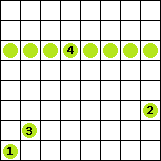
\includegraphics[height=4cm]{pictures/assignment1/Stability.png}
    \caption{Stone 1 has stability 4; Stone 2 has stability 3; Stone 3 and 4 have stability 1}
    \label{fig:Stability}
\end{figure}

Having high stability on one's stones is desirable as it increases the player's chance of retaining his stones until the end. We can calculate the total stability $s$ of a player with the following simple iterative algorithm:

\begin{enumerate}
\item Assign each owned stone stability directions according to directions of neighboring holes
\item Add stability directions to stones that are adjacent to stable stones of the same color
\item Repeat step 2 until no further change occurs
\item Add stability directions to stones that lie on a completely filled horizontal, vertical or diagonal straight line
\item Count stability directions of each stone (0-4)
\item Sum up all stability values to obtain $s$
\end{enumerate}


\subsubsection{Bonus Tiles}
Override stones and bombs are powerful assets that should be deployed strategically. Their valuation are dependent on meta-variables such as map size and bomb radius. A simple heuristic for the value of acquiring 1 additional bomb would be to calculate its area of effect ($\approx (2r+1)^2$) and multiplying the result by 4 since all stones will be completely stable by then. For bonus override stone, it seems reasonable to only use them after the map has been filled by regular moves in order to maximize efficiency. The number of overturned stones is then proportional to $\sqrt{hw}$ where $h, w$ are map height and width - the larger the map, the longer straight line can go. However, both of these heuristics seem to somewhat overestimate: Our bombs will inevitably destroy some of our own stones, and stones captured with override stones can be captured again by other player's override stones. We therefore suggest discounting both bonuses by a factor of 2, leading to following heuristics: 
\[ b_{bomb} = 2(2r+1)^2 \cdot n_{bomb} \quad \quad \quad \quad \quad b_{override} = 2 \sqrt{hw} \cdot n_{override}\]
where $n_{bomb}$ and $n_{override}$ are the number of bombs and override stones in our possession, respectively.
 
\subsubsection{Late Stage}
In the late stage of the Building Phase, with the dwindling number of free tiles (~branching factor) and growing stability of placed stones, the game tree becomes increasingly easy to evaluate. A new heuristic rises to relevance at this point: Clustering, or rather the lack thereof. As stone ownership becomes more and more stable, it becomes viable to consider what effects potential moves have on the second phase of the game. Clearly, clusters of stones provide an easy target for bombs and thus should be avoided. 

Moreover, it now makes sense to differentiate opponents: whereas some opponents are ranked too far above for us to catch up, some opponents are ranked too far below to threaten our rank. Yet it's those that are close in rank to us where the rivalry is the most intense. Of course, the extent of "close" is determined the number of bombs available and their radius - with sufficiently powerful bombs or sufficiently narrow leads everyone might still be in reach. It seems desirable for each of our stone to have as few of our \textbf{\textit{own}} stones and as many of our \textbf{\textit{close-rival's}} stones as possible, to deter attacks on us during the bomb phase. We therefore suggest the following heuristic: \\
\[ l = \sum\limits_{i \in I} c_i \]
where $I$ is the index set of our stones. 
\\
$c_i$ is the "clustering factor" of a particular stone $i$ of ours and is defined by: \\
\[c_i = \frac{\sum\limits_{j=1}^p n_j \cdot r_j}{(2(2r+1)-1)^2}\]
where $p$ is the number of players, $n_j$ is the number of player $j$'s stones within one bomb diameter $(2r+1)^2$ of our stone $i$. \\


\begin{figure}[H]
    \centering
    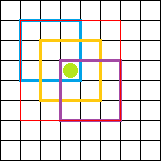
\includegraphics[height=4cm]{pictures/assignment1/Bombing.png}
    \caption{Small $3 \times 3$ squares show possible bombing moves; larger $5 \times 5$ red square shows area the stone is threatened by}
    \label{fig:Bombing Diameter}
\end{figure}

Without loss of generality, let our player number be $1$. \\
$r_j$ is the "rivalry factor" between us and player $j$. We should thus set $r_1$ to $-1$ as we'd like to avoid having our \textbf{\textit{other}} tiles end up as collateral damage of the bombing of our tile $i$. The rest of the $r_j$'s are calculated as: \\
\[r_j = \frac{m_j \cdot (2r+1)^2}{(p-1) \cdot (|N_j - N_1| + 1)} \]
where $m_j$ is the number of bombs available to player $j$; $N_j$ and $N_1$ are the total number of stones of player $j$ and us, respectively. \\
$r_j$ is essentially a measure of how large a fraction of his resources player $j$ has to expend in order to overtake us in ranking. The $+1$ term prevents singularity at $0$, and the $(p-1)$ term normalizes the expression since all else being equal, one would spend $\frac{1}{p-1}$ of their bomb assets on combating each player.


\subsubsection{Building Phase Evaluation function}
Taking everything together, we get the following heuristic functions: \\
\\
Uncertainty Phase: \\
\[h_{uncertain} = b_{bomb} + b_{override} \]
\\
Rest of Building Phase: \\
\[ h_{Build} = m + s + b_{bomb} + b_{override} + 4 \cdot (1-\frac{f}{t}) \cdot l \]
where $f$ is the number of free tiles left and $t$ is the total number of (non-hole) tiles on the map. \\
$(1-\frac{f}{t})$ is a scaling function that regulates the importance of l depending on the stage of the game we're in: In early game most tiles are free and $(1-\frac{f}{t}) \approx 0$, diminishing the importance of the heuristic $l$, whereas in late game $l$ becomes relevant with $(1-\frac{f}{t}) \approx 1$. \\
The factor 4 is due to our other heuristics assigning value 4 to completely stable stones.




\subsection{Bombing phase}
Since we have already been considering the bombing phase in the late stage evaluations of the building phase, we only need to make slight modifications to the expressions derived above to yield a reasonable heuristic for the bombing phase itself: \\
\[{r_j}^{\prime} = \frac{m_1 \cdot (2r+1)^2}{(p-1) \cdot (|N_j - N_1| + 1)} \]
${r_j}^{\prime}$ is almost the same as $r_j$, except we're taking the initiative this time: instead of using the other player's bomb count $m_j$, we're using our own $m_1$. \\
\\
Thus we get: \\
\[c_k = \frac{\sum\limits_{j=1}^p n_j \cdot {r_j}^{\prime}}{(2r+1)^2}\]
\\
And then the entire heuristic for the bombing phase: \\
\[ h_{Bombing} = \sum\limits_{k \in K} c_k \]
where, instead of representing our stones, $K$ is the set of possible moves in our turn.

\end{document}

